\documentclass[fsharpNotes.tex]{subfiles}
\graphicspath{ {./figures/} }

\begin{document}
\chapter{Higher-Order Functions}
\label{chap:higherOrderFunctions}

\abstract{
  A \idx{higher-order function} is a function that takes a function as an argument and/or returns a function. higher-order functions are also sometimes called functionals or functors. In this chapter you will learn how to:
  \begin{itemize}
  \item make functions that take and/or return functions as values.
  \item create new functions with the function composition operator.
  \item create new functions with a partial specification of function arguments.
  \end{itemize}
}

\section{Functions as Values}
F\# is a functions-first programming language with strong support for working with functions as values: Functions evaluate as \idx[closure]{closures}, see \Cref{sec:functions}, which can be passed to and from functions as any other value. An example of a higher-order function is \lstinline{List.map} which takes a function and a list and produces a list, demonstrated in \Cref{higherOrderMap}.
%
\fs{higherOrderListMap}{\lstinline{List.map} is a higher-order function, since it takes a function as argument.}
%
Here \lstinline{List.map} applies the function \lstinline{inc} to every element of the list. higher-order functions are often used together with \idx[anonymous functions]{anonymous functions}, where the anonymous function is given as an argument. For example, \Cref{higherOrderMap} may be rewritten using an anonymous function as shown in \Cref{higherOrderAnonymous}.
%
\fs{higherOrderAnonymous}{An anonymous function is a higher-order function used here as an unnamed argument. Compare with \Cref{higherOrderMap}.}
%

Writing a function that takes other functions as arguments is straightforward. If we were to make our own \lstinline{map} function, it could look like what is shown in \Cref{higherOrderMap}.
%
\fs{higherOrderMap}{A homemade version of \lstinline{List.map}.}
%
In this case, \lstinline{map} has the type
\begin{quote}
  \lstinline{map: f: ('a -> 'b) -> lst: 'a list -> 'b list}
\end{quote}
All three programs result in the same output and as such are equal. Likewise, running times will be equal. However, they differ in readability for a programmer and ease of bug hunting and future maintenance: Bindings allow us to reuse the code at a later stage, but if there is no reuse, then the additional bindings may result in a cluttered program. Nevertheless, programs using anonymous functions can be difficult to debug. Finally, bindings emphasize semantic aspects of the evaluation being performed merely by the names we select, and typically long, meaningful names are to be preferred, within reasonable limits. For example, instead of \lstinline{inc} one could have used \lstinline{increment_by_one} or similar which certainly is semantically meaningful, but many programmers will find that the short is to be preferred in order to reduce the amount of typing to be performed.

Functions can also be return values. For example, in \Cref{higherOrderReturn}, the function \lstinline{incBy} creates functions, which increments by a given argument.
%
\fs{higherOrderReturn}{The procedure \lstinline{inc} returns an increment function. Compare with \Cref{higherOrderMap}.}
%
Note that the closure of this customized function is only produced once when the arguments for \lstinline{List.map} are prepared, and not every time \lstinline{List.map} applies the function to the elements of the list. Compare with \Cref{higherOrderMap}.


\section{The Function Composition Operator}
F\# has strong support for working with functions on a functional level. In \Cref{sec:functions} on page \pageref{page:piping}, we saw how functions can be composed by passing the result of one function to the next, e.g., using piping. Alternatively, we can compose functions before we apply them to values using the \idx[{>>}@\lstinline{>>}]{\lexeme{>>}} and \idx[{<<}@\lstinline{<<}]{\lexeme{<<}} %>> %>> %>>
\idx[composition operator]{composition operators}, which is defined as,
\begin{quote}
  \lstinline{(>>) : ('a -> 'b, 'b -> 'c) -> ('a -> 'c)}\\
  \lstinline{(<<) : ('b -> 'c, 'a -> 'b,) -> ('a -> 'c)} %>>
\end{quote}
i.e., it takes two functions of type \lstinline{'a -> 'b} and \lstinline{'b -> 'c} respectively, and produces a new function of type \lstinline{a' -> 'c}. As an example, consider the composition of the $\log x$ and $\sqrt{x}$ functions to make $f(x) = \log\left(\sqrt{x}\right), x>0$. Using the piping operator, this can be written as \lstinline{x |> sqrt |> log}, which is sufficient, if the function is only to be used once or not passed as an argument. However, the \lexeme{>>} operator allows us to make a new function by \lstinline{logSqrt = sqrt >> log} or equivalently \lstinline{logSqrt = log << sqrt}. %>>
As with the piping operators, the precedence and association rules imply differences in the number of parentheses needed, but in the end, the choice mostly boils down to personal preference. In \Cref{functionPipingAdv} is a comparison of regular composition and the composition operator is shown. 
%
\fs{functionPipingAdv}{A demonstration of differences in function composition.}

\section{Currying}
Functions, with only the initial list of arguments, also return functions. This is called \idx{partial specification} or \idx{currying} in tribute of Haskell Curry\footnote{Haskell Curry (1900--1982) was an American mathematician and logician who also has a programming language named after him: Haskell.}. 
An example is given in \Cref{higherOrderCurrying}.
%
\fs{higherOrderCurrying}{Currying: defining a function as a partial specification of another.}
%
%For functions of more than 1 argument, there exists a short notation which is called \idx{currying} in tribute to Haskell Curry,
Here, \lstinline{mul 2.0} is a partial application of the function \lstinline{mul x y}, where the first argument is fixed, and hence \lstinline{timesTwo} is a function of 1 argument being the second argument of \lstinline{mul}.

Currying is emphasized by how the type of functions of several values is written. Consider a function \lstinline{f} of two generic arguments. Its type in F\# will be \lstinline{f : 'a -> 'b -> 'c}, meaning that \lstinline{f} takes an argument of type \lstinline{'a} and returns a function of type \lstinline{'b -> 'c}. That is, if just one argument is given, then the result is a function, not a value. This is illustrated in \Cref{fig:arrowNotation}.
\begin{figure}
  \centering
  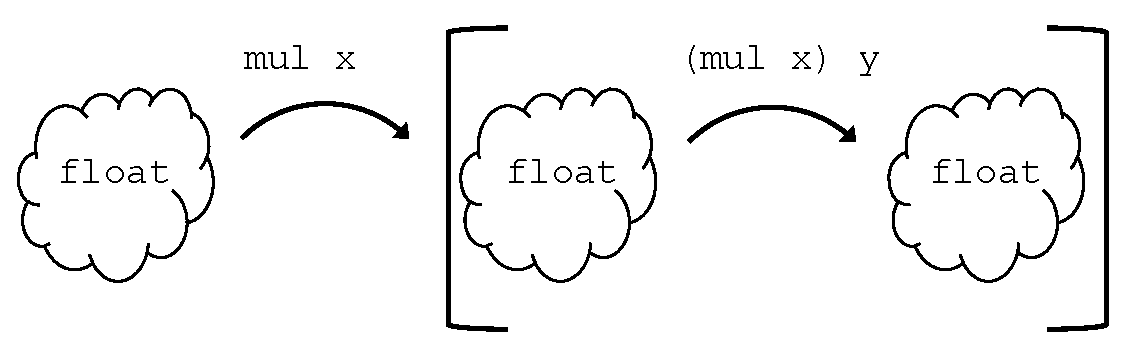
\includegraphics[width=0.6\linewidth]{composition}
  \caption{The type of \lstinline{mul x y = x*y} is a function of 2 arguments is a function from values to functions to values.}
  \label{fig:arrowNotation}
\end{figure}

Currying makes elegant programs and is often used in functional programming. Nevertheless, currying may lead to obfuscation, and in general, \advice{currying should be used with care and be well documented for proper readability of code.}

\section{Key concepts and terms in this chapter}
In this chapter, we have looked at higher-order functions. Key concepts have been:
\begin{itemize}
\item \textbf{Functions are values} and can be used as arguments and return value.
\item Functions can be compose using the \textbf{composition operator} to produce new functions.
\item Function arguments can be \textbf{partially specified} to create new functions with less arguments. This is also called \textbf{currying}.
\end{itemize}
\end{document}
